%Chapter 1 - Intro

\textbf{As I chose a starting point for writing, this has become more of a theory chapter. It will likely be renamed and renumbered to reflect that soon.}

\section{The Quark-Parton Model}
\begin{itemize}
\item Decide how "historical" to be
\item Hadrons are composed of quarks
\item Quarks are bound by gluons (strong force)
\item Gluons create the "sea" via $g\rightarrow q\bar{q}\rightarrow g$
\item Electric and Magnetic form factors?
\end{itemize}

The Quark-Parton Model describes the composition of hadrons, both baryons and mesons. Prior to 1964, it was believed that hadrons were as small as it got. However, the adherence of hadrons to the eight-fold way, a categorization of hadrons by charge and strangeness, suggested that there was some underlying mechanism that had yet to be discovered.

In 1964, Gell-Mann and Zweig independently suggested that hadrons could be composed smaller elementary particles. Gell-Mann offered the name "quarks" for these constituents.

Furthering the theory, in Novemeber 1974 two separate experiments published the discovery of the (now named) $J/\psi$ particle. The long lifetime of the $J/\psi$ suggested that new physics must be at play. The Quark-Parton Model predicted the existence of a quark symmetric to the strange quark, called the charm quark. It was determined that the $J/\psi$ could be a meson comprised of a charm and anti-charm, suggesting the validity of the model.

\section{Deep Inelastic Scattering}
\textbf{How does it work?}
Electron comes in, exchanges photon with nucleon. Boom.

At its most basic, Deep Inelastic Scattering (DIS) is the scattering of a lepton from a nucleon. The two participants exchange a virtual boson, the lepton scatters, and the nucleon is excited to a hadronic final state $X$ with higher mass.

\begin{equation*}
	\ell + N \rightarrow \ell^\prime + X
\end{equation*}

For the MARATHON experiment we will focus on electromagnetic DIS. In this case the lepton is charged and the exchanged virtual boson is a virtual photon. The JLab CEBAF accelerator provides an electron beam, so from here on the lepton will be written as an electron.

\begin{equation*}
	e^- + N \rightarrow e^- + X
\end{equation*}

\textbf{PUT DIS FEYNMAN DIAGRAM HERE}

By interacting with a single nucleon, DIS is a powerful tool for studying nucleon structure. By looking at the DIS cross section, we can see how the nuclear structure functions readily present themselves.

If we assume Lorentz invariance, \textbf{P} and \textbf{T} invariance, and conservation or lepton current, the cross section is

\begin{equation}
	\frac{d^2\sigma}{d\Omega dE^\prime} = \frac{\alpha^2}{Q^4}\frac{E^\prime}{E} L^{\left(s\right)^{\mu\nu}}W^{\left(s\right)}_{\mu\nu}
\end{equation}

where $Q^2$ is the 4-momentum transfer, $E$ is the beam energy, $E^\prime$ is the scattered electron energy, $L^{\left(s\right)^{\mu\nu}}$ is the lepton tensor, and $W^{\left(s\right)}_{\mu\nu}$ is the symmetric hadronic tensor.

When written explicitly in the laboratory frame, we arrive at

\textbf{DIS Cross Section}

\begin{equation}
	\sigma \equiv \frac{d^2\sigma}{d\Omega dE^\prime}\left(E,E^\prime,\theta\right) = \frac{4\alpha^2\left(E^\prime\right)}{Q^4}\cos^2\left(\frac{\theta}{2}\right)\left[\frac{F_2\left(\nu,Q^2\right)}{\nu}+\frac{2F_1\left(\nu,Q^2\right)}{M}\tan^2\left(\frac{\theta}{2}\right)\right]
\end{equation}

\section{$F_2$ Structure Functions}
"These two form factors, $F_{1,2}(q^2)$, parametrize our ignorance of the detailed structure of the proton". \cite{HaM}

\textbf{TALK MORE ABOUT THIS RELATION}

The following relation allows the cross section to be written in terms of $F_2$ only.

\begin{equation}
	F_1 = \frac{F_2\left(1+Q^2/\nu^2\right)}{2x\left(1+R\right)}
\end{equation}

Here $x$ is the bjorken scaling variable and $R$ is the ratio of the longitudinal cross section to the transverse cross section, $\sigma_L/\sigma_T$.

Plugging this in we arrive at

\begin{equation}
	\frac{d^2\sigma}{d\Omega dE^\prime}\left(E,E^\prime,\theta\right) = \frac{4\alpha^2\left(E^\prime\right)}{Q^4}\cos^2\left(\frac{\theta}{2}\right)F_2\left[\frac{1}{\nu}+\frac{\left(1+Q^2/\nu^2\right)}{xM\left(1+R\right)}\tan^2\left(\frac{\theta}{2}\right)\right]
\end{equation}

\section{$R=\sigma_L/\sigma_T$}
\textbf{$R=\sigma_L/\sigma_T$. $R$ is independent of atomic number. This facilitates us taking ratios}

If we instead approach DIS as the production and absorption of a virtual photon by a parton we can extract a different structure function $R=\sigma_L/\sigma_T$, referred to as photonuclear R. That is, the ratio of the cross sections for absorbing longitudinal photons to transverse photons.

We can write the DIS cross section in terms of these cross sections as

\begin{equation}
	\frac{d^2\sigma}{d\Omega dE^\prime}\left(E,E^\prime,\theta\right) = \Gamma\left[\sigma_T\left(x,Q^2\right)+\epsilon\sigma_L\left(x,Q^2\right)\right]
\end{equation}

In this equation $\Gamma$ is the flux of transverse virtual photons and $\epsilon$ is the relative flux of longitudinal virtual photons. These are defined by

\begin{equation}
	\Gamma = \frac{\alpha KE^\prime}{2\pi^2Q^2E_0\left(1-\epsilon\right)}
\end{equation}

\begin{equation}
	\epsilon = \frac{1}{1+2\left(1+\nu^2/Q^2\right)\tan^2\left(\frac{\theta}{2}\right)}
\end{equation}

Here, $K$ is the laboratory photon energy

\begin{equation}
	K = \frac{W^2-M^2}{2M}
\end{equation}

In this schema we find that:

\begin{equation}
	F_1 = \frac{F_2\left(1+Q^2/\nu^2\right)}{2x\left(1+R\right)}
\end{equation}

Substituting this into our DIS cross section equation, we can eliminate $F_1$. This also makes it clear that we can easily access the $F_2$ structure functions by measuring cross section ratios.

\begin{equation}
	\frac{d^2\sigma}{d\Omega dE^\prime}\left(E,E^\prime,\theta\right) = \frac{4\alpha^2\left(E^\prime\right)}{Q^4}\cos^2\left(\frac{\theta}{2}\right)F_2\left[\frac{1}{\nu}+\frac{\left(1+Q^2/\nu^2\right)}{xM\left(1+R\right)}\tan^2\left(\frac{\theta}{2}\right)\right]
\end{equation}

If we measure the cross section ratios of two different targets, we find:

%\begin{equation}
%	\frac{\sigma_A}{\sigma_B} = \frac{F_2^A\left[1 + }{•}
%\end{equation}

Historical data suggests that photonuclear R has no nuclear dependence to within $10\%$. If we assume that that there is no nuclear dependence, this equation simplifies to:

\begin{equation}
	\frac{\sigma_A}{\sigma_B} = \frac{F_2^A}{F_2^B}
\end{equation}

\section{EMC Ratios}
\textbf{Looking at the EMC-type ratios for Helium-3 and Tritium make it clear that we can extract the nucleon structure function ratio from the nuclear structure function ratio. We will use a calculation of the super ratio to do this extraction.}

%\subsection{First subsection}
%
%This is the first subsection of the first section of the first Chapter....
%
%
%\begin{table}[ht]
%\caption{Quarks, Leptons and Gauge Bosons}			% title of Table
%\centering										% used for centering table
%\begin{tabular}{l c c c r}							% centered columns (5 columns)
%\hline										%inserts single horizontal line
%Generation		& Quark 						& Electric Charge($\left | q_{e} \right |$)	& Mass($MeV/c^{2}$)	& Spin\\ 	 	% inserts table
%\hline										% inserts single horizontal line
%First				&Up (u)						& +2/3							& 1.7-3.1				& 1/2\\	%insertingbodyofthetable
%				& Down (d)					& -1/3							& 4.1-5.7				& 1/2\\[1ex]
%Second			& Charm (c)					& +2/3							& 1180-1340			& 1/2 \\
%				& Strange (s)					& -1/3 							& 80-130				& 1/2 \\[1ex]
%Third				& Top (t)						& +2/3 							& 172900$\pm$1500	& 1/2 \\
%				& Bottom (b) 					& -1/3		 					& 4130-4370			& 1/2 \\ [1ex]% [1ex] adds vertical space 
%\hline
%Generation		& Lepton						& Electric Charge($\left | q_{e} \right |$)	& Mass($MeV/c^{2}$)	& Spin\\ 
%\hline
%First				& Electron (e)					& -1								& 0.511				& 1/2\\
%				& Electron Neutrino ($\nu_{e}$)	& 0								& 0					& 1/2\\[1ex]
%Second			& Muon ($\mu$)				& -1								& 105.66				& 1/2\\
%				& Muon Neutrino ($\nu_{\mu}$)	& 0								& 0					& 1/2\\[1ex]
%Third				& Tau ($\tau$)					& -1								& 1776.84				& 1/2\\
%				& Tau Neutrino ($\nu_{\tau}$)		& 0								& 0					& 1/2\\[1ex]
%\end{tabular}
%\begin{tabular}{c c c c c}
%\hline
%Force			& Gauge Boson				& Electric Charge($\left | q_{e} \right |$)	& Mass($GeV/c^{2}$)	& Spin\\ 
%\hline
%Electromagnetic	& $\gamma$ (Photon)			& 0								& 0					& 1\\[1ex]
%Weak Nuclear		& $W^{\pm}$					& $\pm 1$							& 80.3980$\pm$0.025	& 1\\
%				& $Z^{0}$						& 0								& 91.1876$\pm$0.0021	& 1\\[1ex]
%Strong Nuclear		& g (8 Gluons)					& 0								& 0					& 1\\[1ex]
%\hline
%\end{tabular}
%\label{table:nonlin}								% is used to refer this table in the text
%\end{table}
%
%\newpage 
%
%
%\subsection{Second subsection}
%
%This is the second subsection....
%
%Here comes a Figure......
%
% \begin{figure}[!htbp]
%  \begin{center}
%    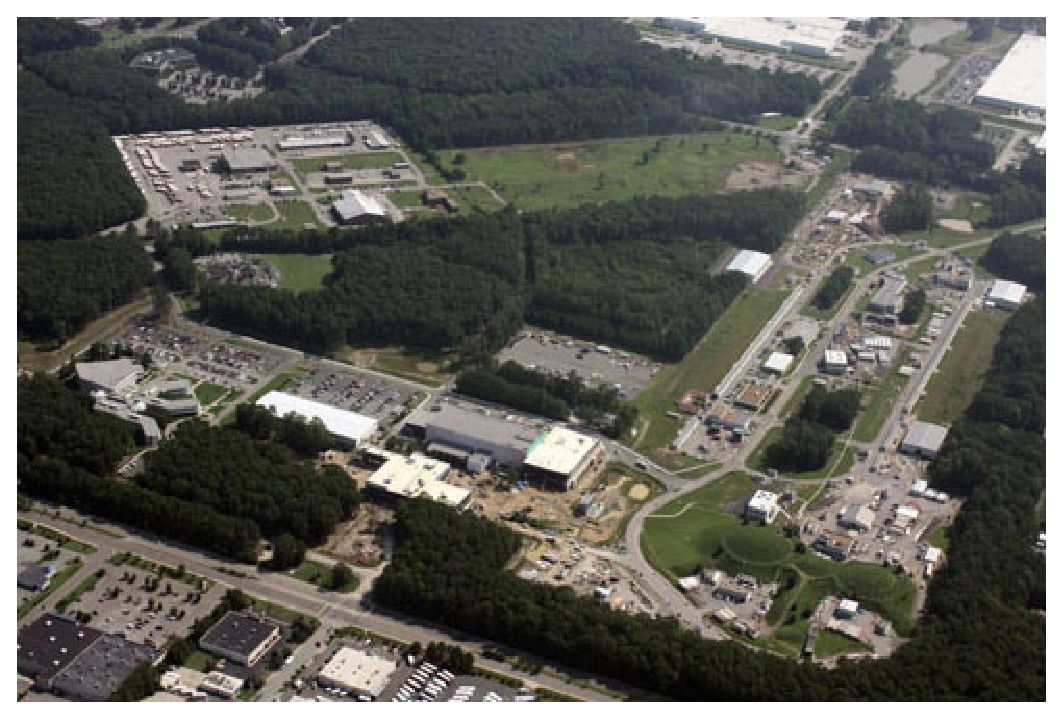
\includegraphics[angle=0, scale=0.85]{./chap1-intro/fig/Visit-JLab3.eps}
%  \end{center}
%  \caption[Aerial view of Jefferson Laboratory, Newport News, Virginia.]{
%    \footnotesize Aerial view of JLab
%  }
%  \label{fig:AerJLab}
%\end{figure}
%
%
%
%Use the label name to refer to  Figure  ~\ref{fig:AerJLab}.
%
%\subsubsection{Sub sub section a}
%
%This is a subsubsection
%
%\subsubsection {Sub sub section b}
%
%Another subsubsection......

